
\documentclass[runningheads]{llncs}
\usepackage{graphicx}
\usepackage{apacite}
\usepackage{float}
\usepackage{listings}
\lstset{
  basicstyle=\ttfamily,
  columns=fullflexible,
  frame=single,
  breaklines=true,
  postbreak=\mbox{\textcolor{red}{$\hookrightarrow$}\space},
}
\usepackage{float}
\usepackage[table]{xcolor}
\usepackage[toc,page]{appendix}
\usepackage{ucs}
\usepackage[utf8x]{inputenc}

\usepackage{hyperref}
\hypersetup{
	colorlinks=true,
	linkcolor=blue,
	filecolor=magenta,      
	urlcolor=cyan,
}

\usepackage[slovene]{babel}
\selectlanguage{slovene}

\lstset{
    breaklines=true,
    breakatwhitespace=true,
    inputencoding=utf8,
    extendedchars=false,
}

\renewcommand{\baselinestretch}{1.2} % za boljšo berljivost večji razmak
\renewcommand{\appendixpagename}{\normalfont\Large\bfseries{Appendix}}

\begin{document}

\title{Seminarska naloga}
\subtitle{Implementacija algoritma za grupiranje in določanja vodja grupe}

\author{Danijel Maraž, Nejc Rebernik}

\institute{Fakulteta za Računalništvo in Informatiko UL
\email{dm9929@student.uni-lj.si}\\
}

\maketitle             

\begin{abstract}
The article covers the work done in the scope of the seminar assignment as part of the subject wireless sensor networks.

\keywords{Raft nRF24LO1 Leader Consensus Wemos ESP}
\end{abstract}

\section{Uvod}
TODO tukaj povedat ključne cilje projekta 

Cilj projekta je bila implementacija algoritma za določanje vodje v gruči naprav v brezžičnem omrežju.

Razvoj in testiranje sva opravljala na ploščici z WEMOS D1 mini kontrolerjem in modulom za komuniciranje nRF24L01. Na ploščici so bili nameščeni še drugi moduli, ki pa jih v obsegu najinega razvoja nisva uporabila. Modul nRF24L01 sprejema in oddaja na frekvenci 2.4GHz z maksimalno hitrostjo prenosa do 2Mbps. Majhne velikosti sporočil uporabljenih v komunikaciji in glede na to relativno velika podatkovna pretočnost sta omogočala hiter razvoj in testiranje ter skalabilnost.

Za določanje vodje v gruči sva implementirala protokol RAFT. Programska koda je napisana v jeziku C++ s knjižnico za upravljanje s komunikacijskim modulom nRF24L01.

\section{Splošna struktura}
splošen opis kode

Glavni implemetacijski nalogi sta bili implementacija RAFT algoritma ter pošiljanje in prejemanje podatkov. Podrobnosti RAFT protokola in implementacije so opisane v temu namenjenemu poglavju. 

RAFT protokol temelji na robustni distribuirani strukturi volitev.

\subsection{Election task}
opis taska, čemu služi itd. slikica

Volitve so prvi izmed korakov v iskanju novega vodje gruče v primeru kjer vodja ni določen oziroma je prišlo do izpada trenutnega vodje. Vsaka naprava ima interni naključni časovnik ki sproži signal za začetek volitev. Namen volitev je implicitno sporočanje da vodja gruče v tem času ni določen in iskanje novega vodje gruče.
\subsection{Listen and react task}
opis delovanja taska slikica
\subsection{Device table}
kako deluje device table glej funkcije

Tabela naprav je namenjena shranjevanju seznama naprav in stanja naprav v omrežju. Vsaka naprava dodana v omrežje se zapiše v lokalno tabelo naprav in odstrani ob odstranitvi iz omrežja.
\section{nRF24}
tukaj povedat kako poteka komunikacija s pomočjo modula:
bistvo je da se auto acknowledgement paketki ne avtomatsko pošiljajo in konstantno odpiramo pa zapiramo write in listen pipe da doseženo učinek broadcasta

Na ploščici je nameščen modul za komuniciranje nRF24L01. Modul deluje na frekvenci 2.4GHz. Za krmiljenje je na voljo knjižnica v jeziku C.

Modul je deloval zanesljivo na kratkih razdaljah reda velikosti nekaj metrov. Delovanje na večjih razdaljah je možno doseči z uporabo dodatne antene.

Z vidika programske opreme je priložena knjižnica dobro dokumentirana. Največji izziv pri uporabi modula je bilo sočasno prejemanje in oddajanje.

Prvotno sva za prejemanje in oddajanje ustvarila dva taska, kar se je kasneje izkazalo za neučinkovito, ker je prihajalo do zakasnitev in nedostavljenih paketov zaradi nesinhroniziranosti. Kasneje sva izziv rešila z uporabo enega taska, ki je ves čas v načinu poslušanja, ki pa se začasno spremeni v način pošiljanja, ko želimo poslati sporočilo. S tem pristopom sva bistveno zmanjšala število izgubljenih paketov in prihranek na energiji, saj modul v načinu oddajanja porabi več energije.

\section{Raft}
opis rafta, vključi tudi robne primere ko vodja ni izvoljen ker ni dovolj glasov

RAFT protokol temelji na robustni distribuirani strukturi volitev. Na začetku se naprave v gruči ne zavedajo drugih naprav, niti nimajo določenega vodje. S periodičnimi sporočili si sestavijo tabelo naprav v okolici in določijo vodjo gruče.

RAFT, kot drugi algoritmi za doseganje konsenza uporablja timerje, pri čemer se razlikuje v tem, da ima vsaka naprava naključno določen interval komuniciranja, kar pospeši reševanje konfliktov v algoritmu.

\section{Protokol komunikacij}
\begin{figure}
  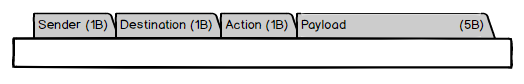
\includegraphics[width=\linewidth]{packet.png}
  \caption{Osnovna oblika paketa.}
  \label{fig:paket}
\end{figure}
slika paketka, v glavnem je maksimalen payload 8 bajtov na eno komunikacijo zato smo prve 3 rezervirali za naš addressing ostale pa za namišljen payload ki bi ga imeli v realni situaciji.
prvi bajt je zadnja črka MAC addressa ploščice, ki pošilja. drugi nam pove komu je pošiljka (F za broadcast) namenjena. tretji pa je funkcijski pomen, akcija E za election V za oddat glas A za acknowledge heartbeat H za heartbeat itd.
\section{One time pad}
opis one time pad. zakaj smo si ga izbrali (ker je simple). opis kako bi se dalo razbit vsebino komunikacij. imam samo en stalen ključ, ker bi bilo ponovno izmenjevanje preveč zapleteno gleda na nivo fleksibilnosti, ki ga imamo v našem sistemu wemosov.
\section{Primeri}
\begin{figure}
  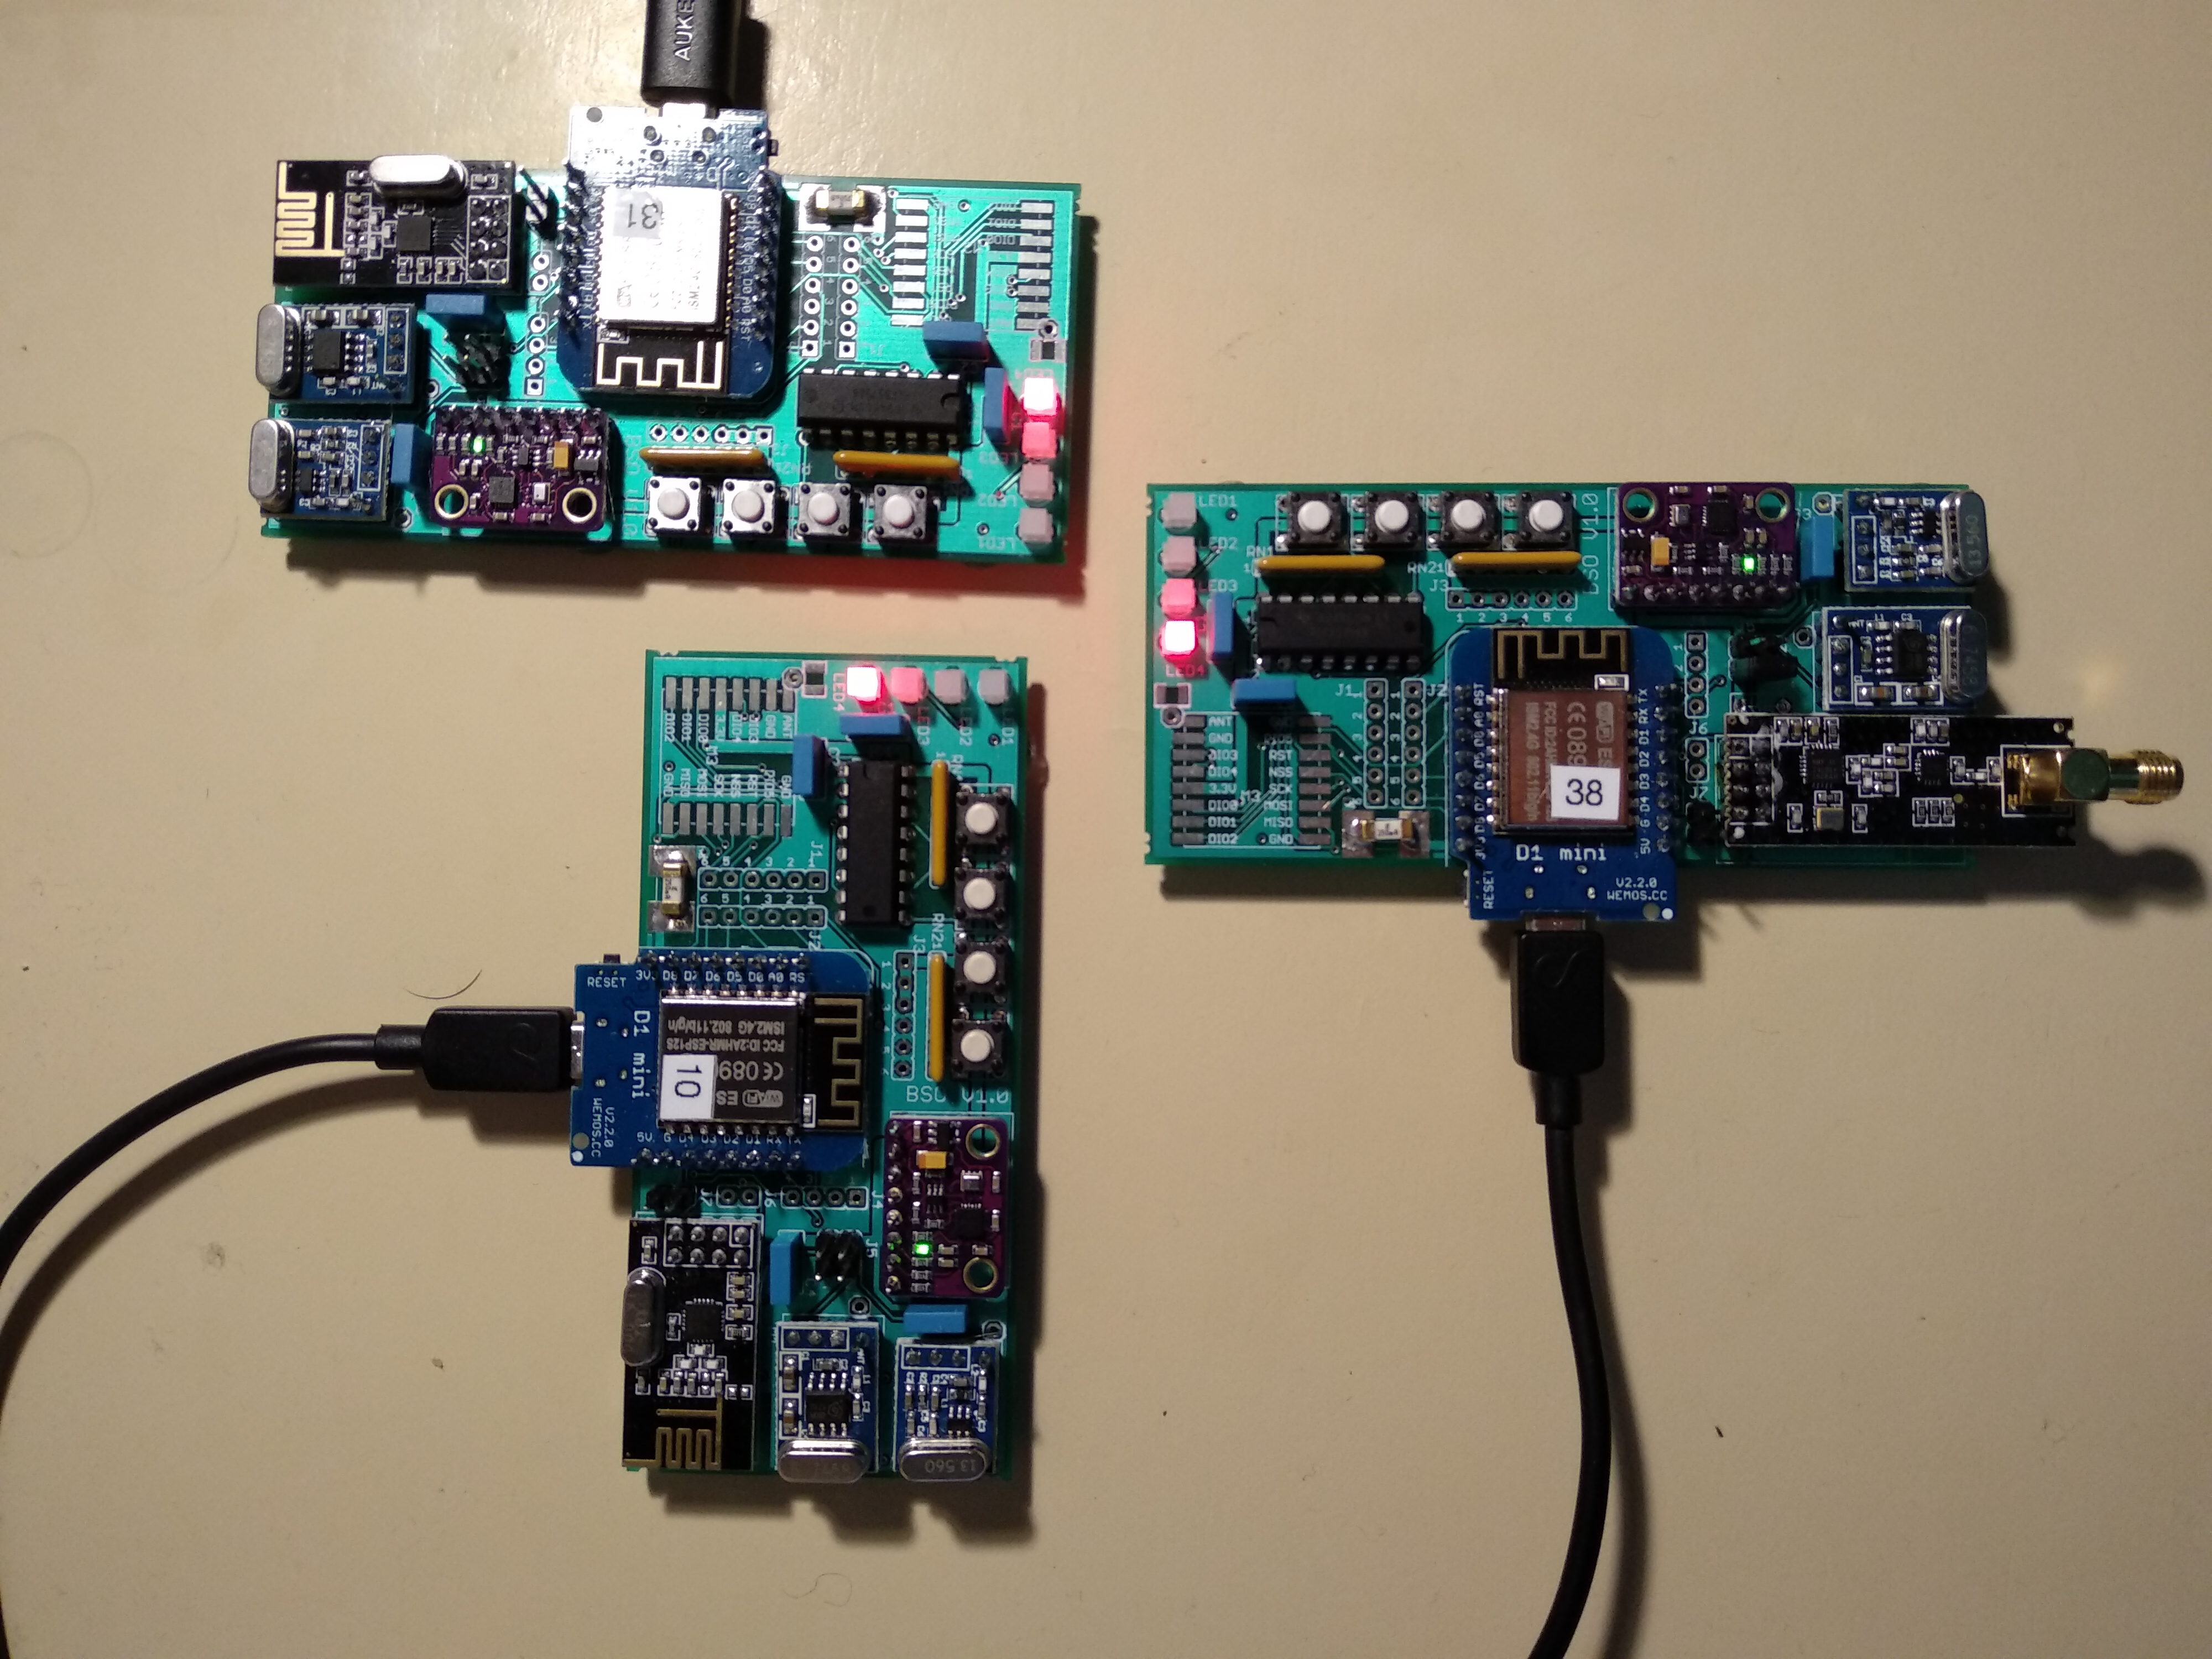
\includegraphics[width=\linewidth]{no_leader.jpg}
  \caption{Brez vodje bodo kmalu sledile nove volitve.}
  \label{fig:no_leader}
\end{figure}
\begin{figure}
  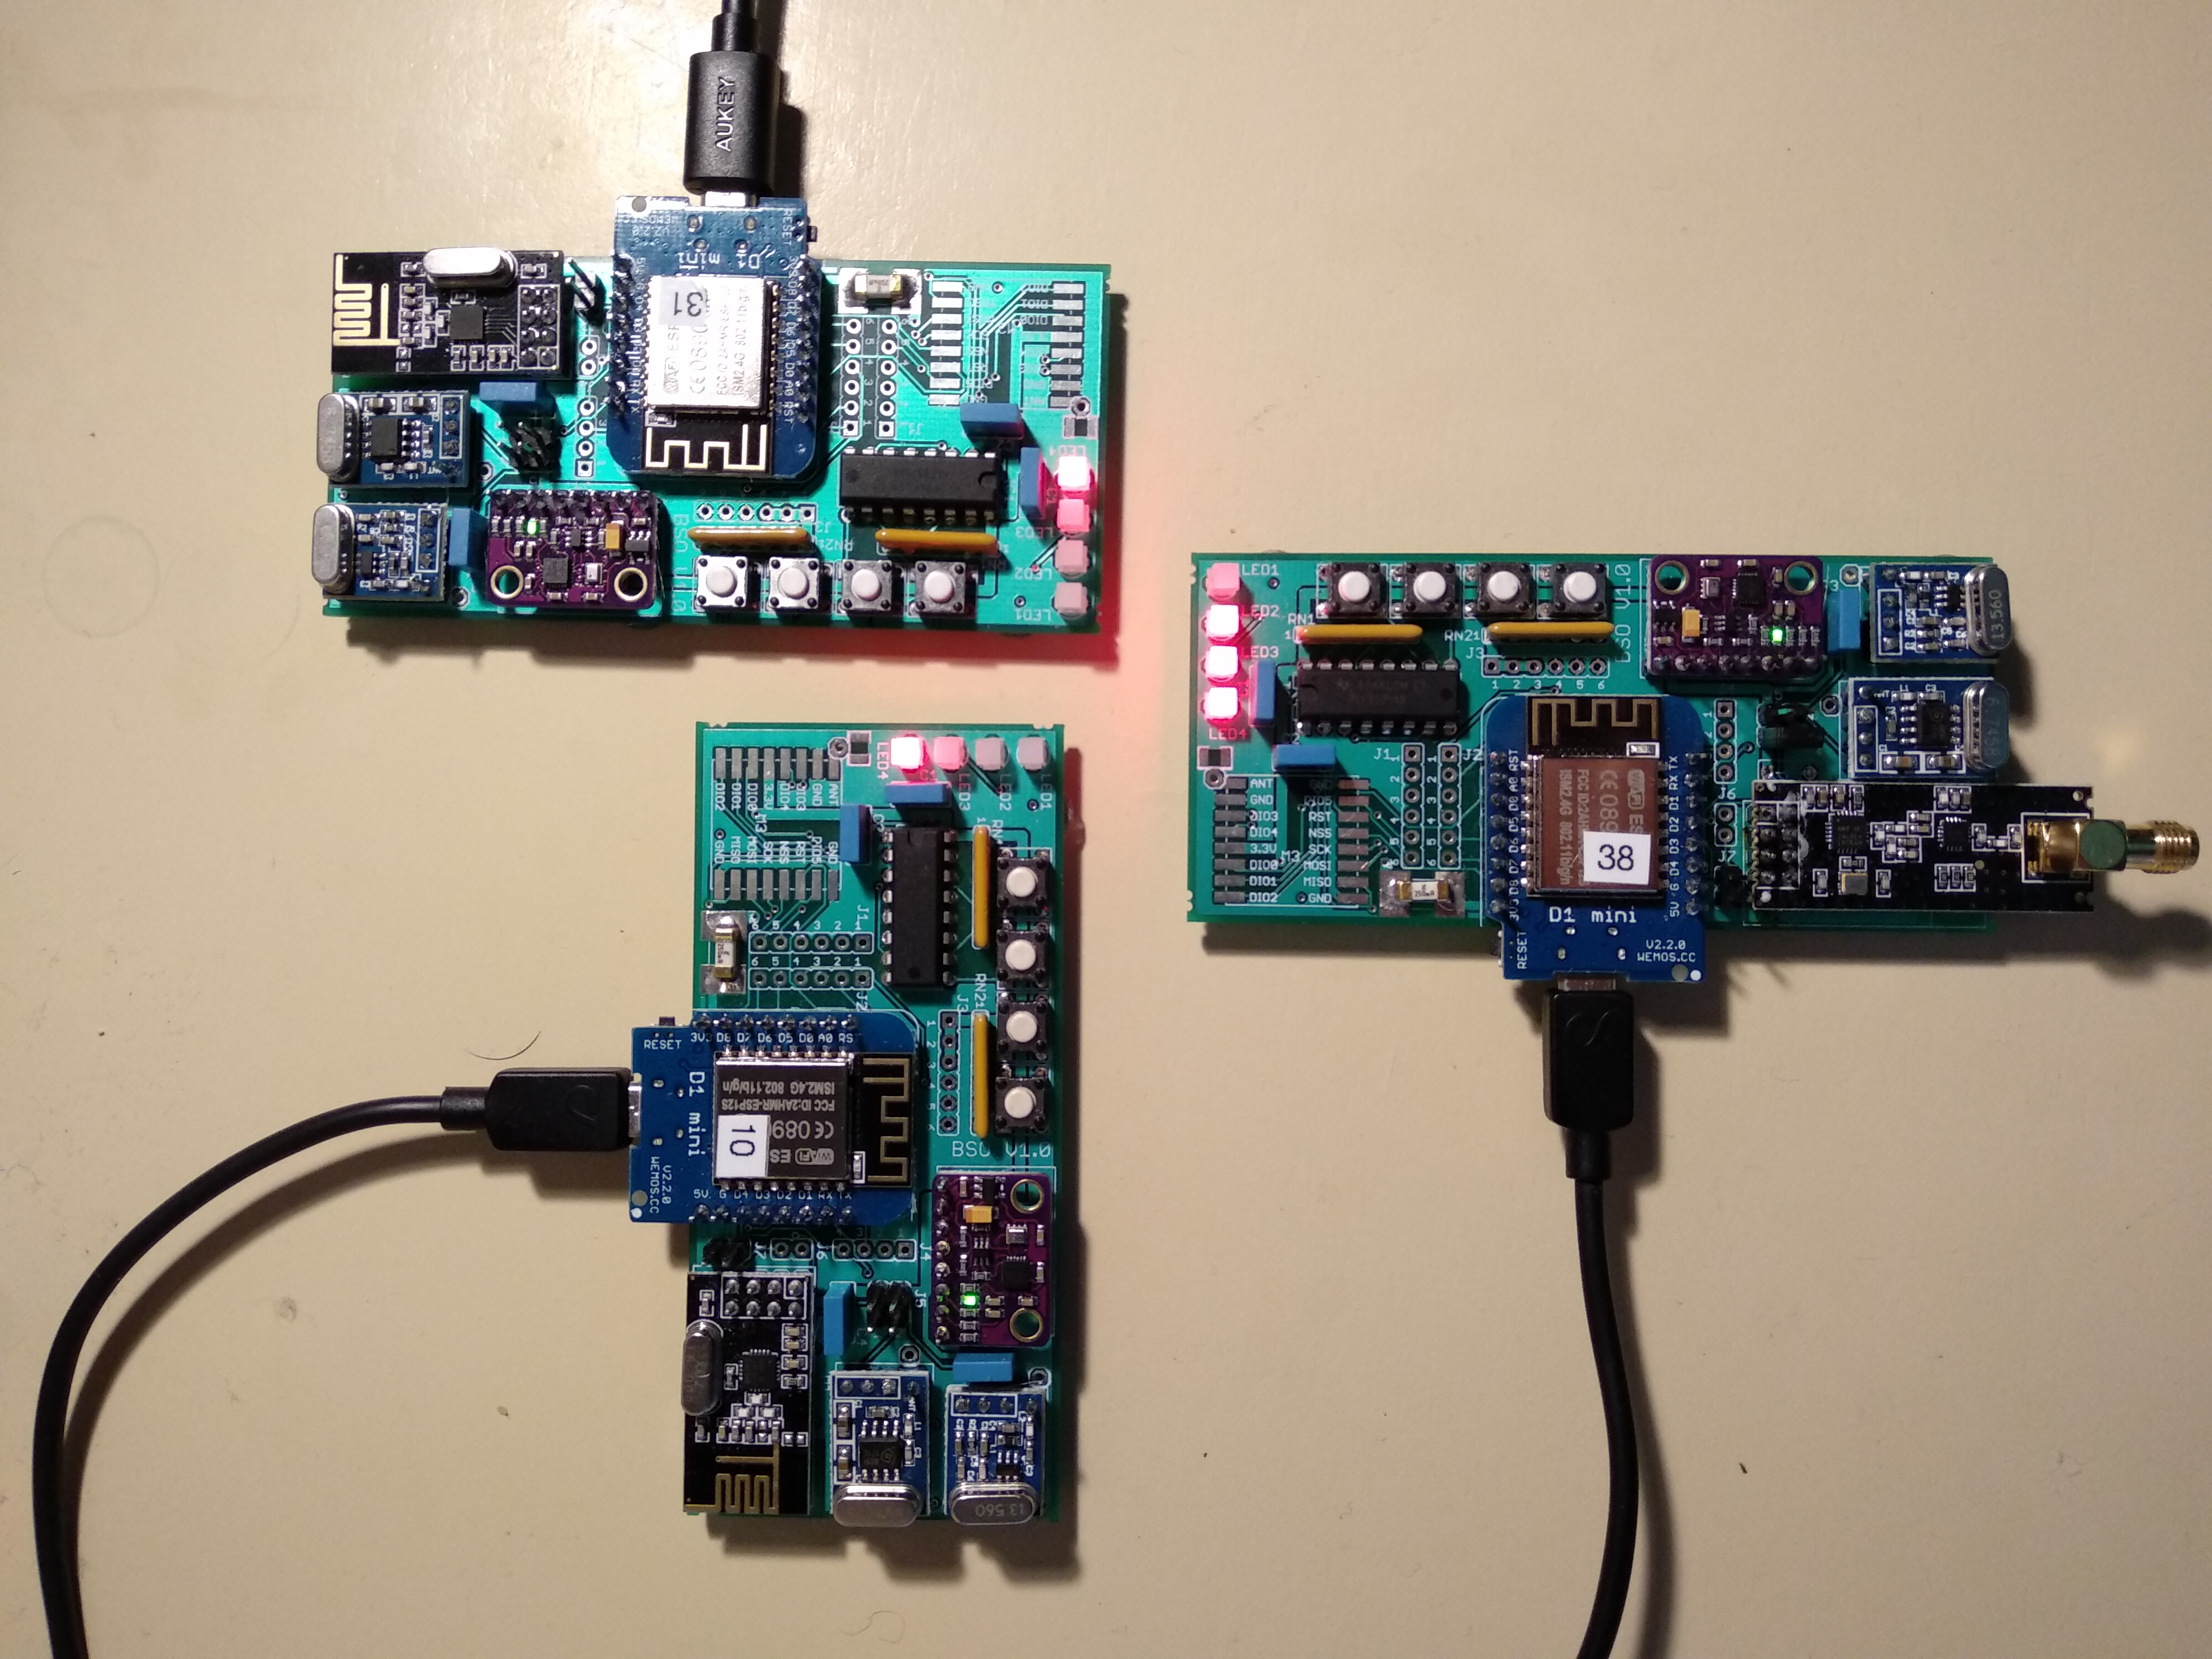
\includegraphics[width=\linewidth]{one_leader.jpg}
  \caption{Prisotnost vodje.}
  \label{fig:one_leader}
\end{figure}

\section{Zaključek}
dosežki projekta:
-delujoč določanje vodje (Raft)
-samo 1 preprosta koda za vsako napravo
-naprave se lahko poljubno priključijo v omrežje
-enkripcija one time pad
\end{document}

